\chapter{Design Method: From a Vague Idea to Twelve Falsifiable Decisions}\label{ch:design}

\begin{objectives}
After this chapter you should be able to:
\begin{itemize}
\item describe the state of \texttt{score} before the extension, and name its three structural gaps;
\item explain what makes a design decision \emph{falsifiable}, and write a falsifier for each of the twelve decisions;
\item explain the ``decision frontier'' technique a grilling session uses to order questions;
\item argue, with a counting argument, why the extension was built as interfaces first;
\item justify scaffolding with stubs that \emph{throw} rather than stubs that return defaults.
\end{itemize}
{\small\color{muted}\textbf{Chapter references:} Parnas~\cite{parnas1972criteria}; Martin~\cite{martin2003agile}; Gamma et al.~\cite{gamma1994design};
Brooks~\cite{brooks1975mythical}.}
\end{objectives}

\section{Where the repository started}\label{sec:start}
\texttt{score} is a C++23 shared library, \texttt{libscore\_core}, with a C API and nanobind bindings to a Python
package. Before this work it computed descriptive statistics, log-returns, a Sharpe ratio and maximum drawdown
(\cref{fig:arch}). It had three structural gaps, and every later chapter grows out of one of them.

\begin{enumerate}[label=\textbf{\color{yel}G\arabic*.}]
\item \textbf{No persistence.} Prices entered through two unconnected paths: live pulls from \texttt{yfinance}
(\cref{lst:market}) and a synthetic geometric-Brownian-motion generator (\cref{lst:gbm}). Neither stored anything that a
later query could read.
\item \textbf{No tail-risk measure.} The library could say how volatile a stock was, but not how bad a bad day is.
That question is answered by Value at Risk and Expected Shortfall.
\item \textbf{No networking or concurrency.} Nothing could serve a request from another process.
\end{enumerate}

\begin{figure}[htbp]
\centering
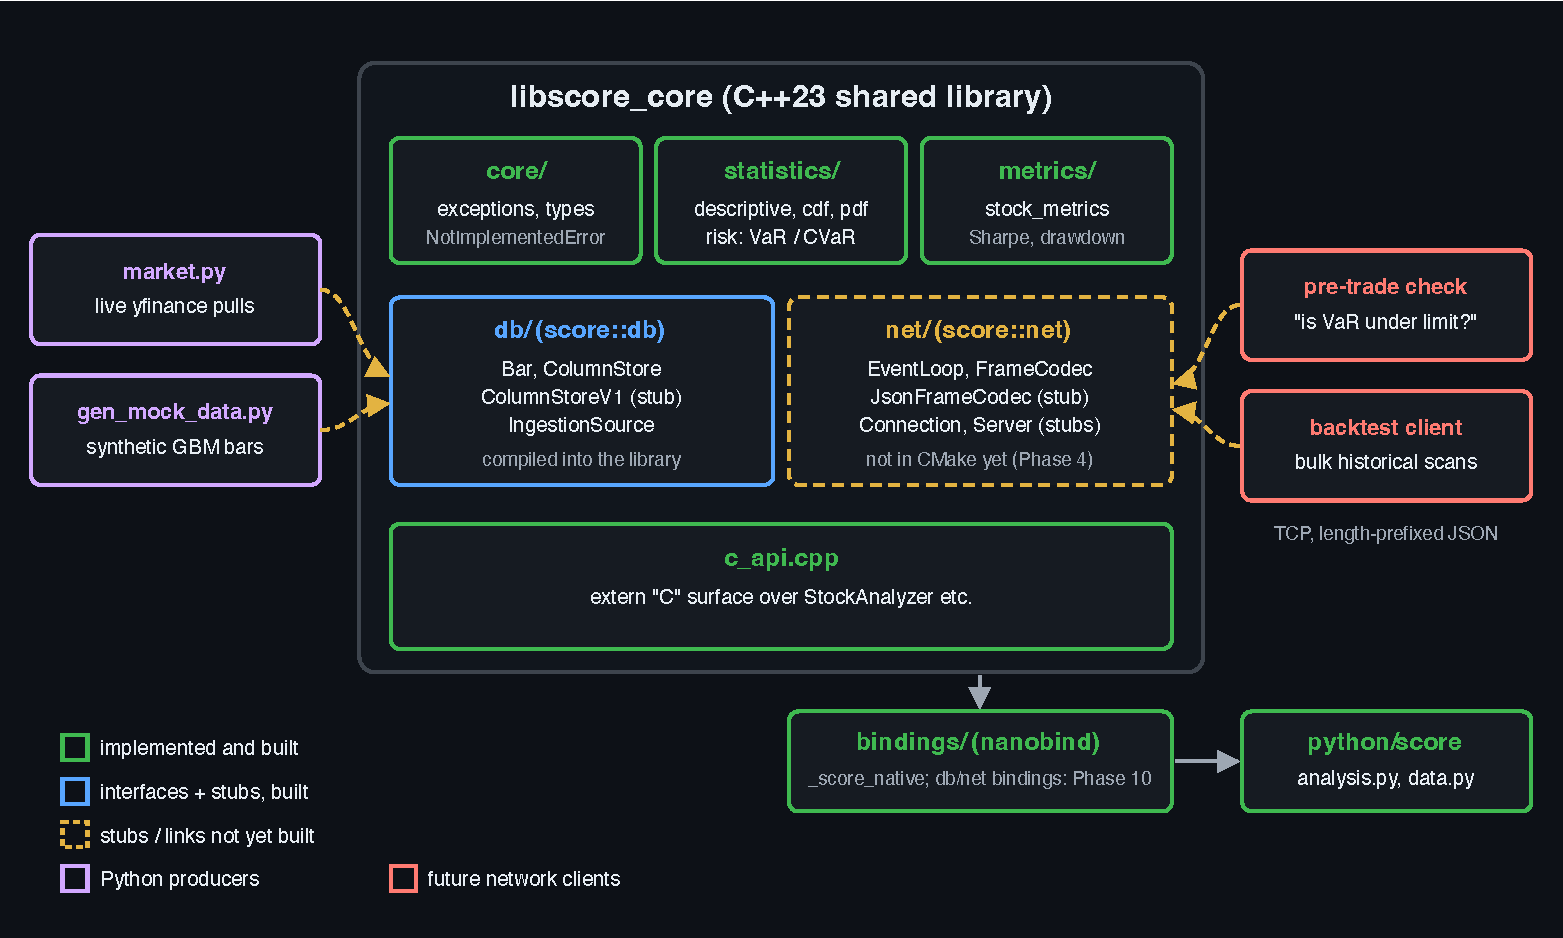
\includegraphics[width=\linewidth]{diagrams/architecture.pdf}
\caption{Module map of \texttt{score} after Phases 0--3 (hand-authored SVG). \texttt{db/} is compiled into the library;
\texttt{net/} exists as headers and stubs but is deliberately not yet in the CMake source list (Phase~4, \cref{ch:roadmap}).}
\label{fig:arch}
\end{figure}

\repopy{src/score/market.py}{\textbf{Data path 1.} \cc{MarketData} wraps \cc{yfinance} and caches one daily-history fetch.
Note \cc{period="1d"}: this facade fetches a single day, so it cannot supply the hundreds of returns a historical VaR
needs. \Cref{ex:yf} asks what \cc{ingest()} must change.}{lst:market}

\repopy[firstline=74,lastline=80]{scripts/gen_mock_data.py}{\textbf{Data path 2} (lines 74--80). The path is the exact
log-space GBM recursion $S_{t+1}=S_t\exp\big((\mu-\tfrac12\sigma^2)\Delta t+\sigma\sqrt{\Delta t}\,Z\big)$ with
$\Delta t=1/252$ (\cref{sec:gbm}). The output is written to JSON and is never read back by the C++ side.}{lst:gbm}

\section{Grilling: interviewing a design into existence}
The request that started this work was roughly ``add a database and some networking, so I can learn''.
That sentence admits thousands of designs, from ``install PostgreSQL and gRPC'' to ``write a kernel-bypass engine''.
A \emph{grilling session} is a structured interview that narrows the space by asking one question at a time,
always with a recommended answer and a reason, until every remaining question has an obvious answer.

\begin{layman}
A good doctor taking a history does not ask every question in the textbook. Each answer prunes the tree:
``does it hurt when you breathe?'' makes some questions urgent and others irrelevant. The doctor also
proposes a working diagnosis at every step, so the patient can say ``no, that's not it''. A grilling session is the
same: each question comes with a proposed answer you can reject.
\end{layman}

\begin{definition}[Decision; falsifier]\label[definition]{def:decision}
A \emph{design decision} is a tuple $(q, A, a^\star, \phi)$: a question $q$, a set of alternatives $A$, the chosen
alternative $a^\star\in A$, and a \emph{falsifier} $\phi$, an observable condition that, if it held, would make some
$a\in A\setminus\{a^\star\}$ the better choice. A decision without a falsifier is a preference, not a decision.
\end{definition}

\begin{definition}[Dependency order and frontier]\label[definition]{def:frontier}
Write $q_i\prec q_j$ if the answer to $q_i$ changes the alternatives available for $q_j$. Given the set $R$ of resolved
questions, the \emph{frontier} is $\mathcal{F}(R)=\{q\notin R:\ \forall p\prec q,\ p\in R\}$.
\end{definition}

The session's one rule is \emph{always ask from the frontier}. Asking a question before its predecessors are settled
wastes the answer: ``epoll or io\_uring?'' is meaningless until ``hand-rolled TCP or gRPC?'' is answered. Because
$\prec$ is acyclic, the frontier is never empty while questions remain, and asking from it is a topological traversal
of the decision graph (\cref{fig:grill}).

\begin{figure}[p]
\centering
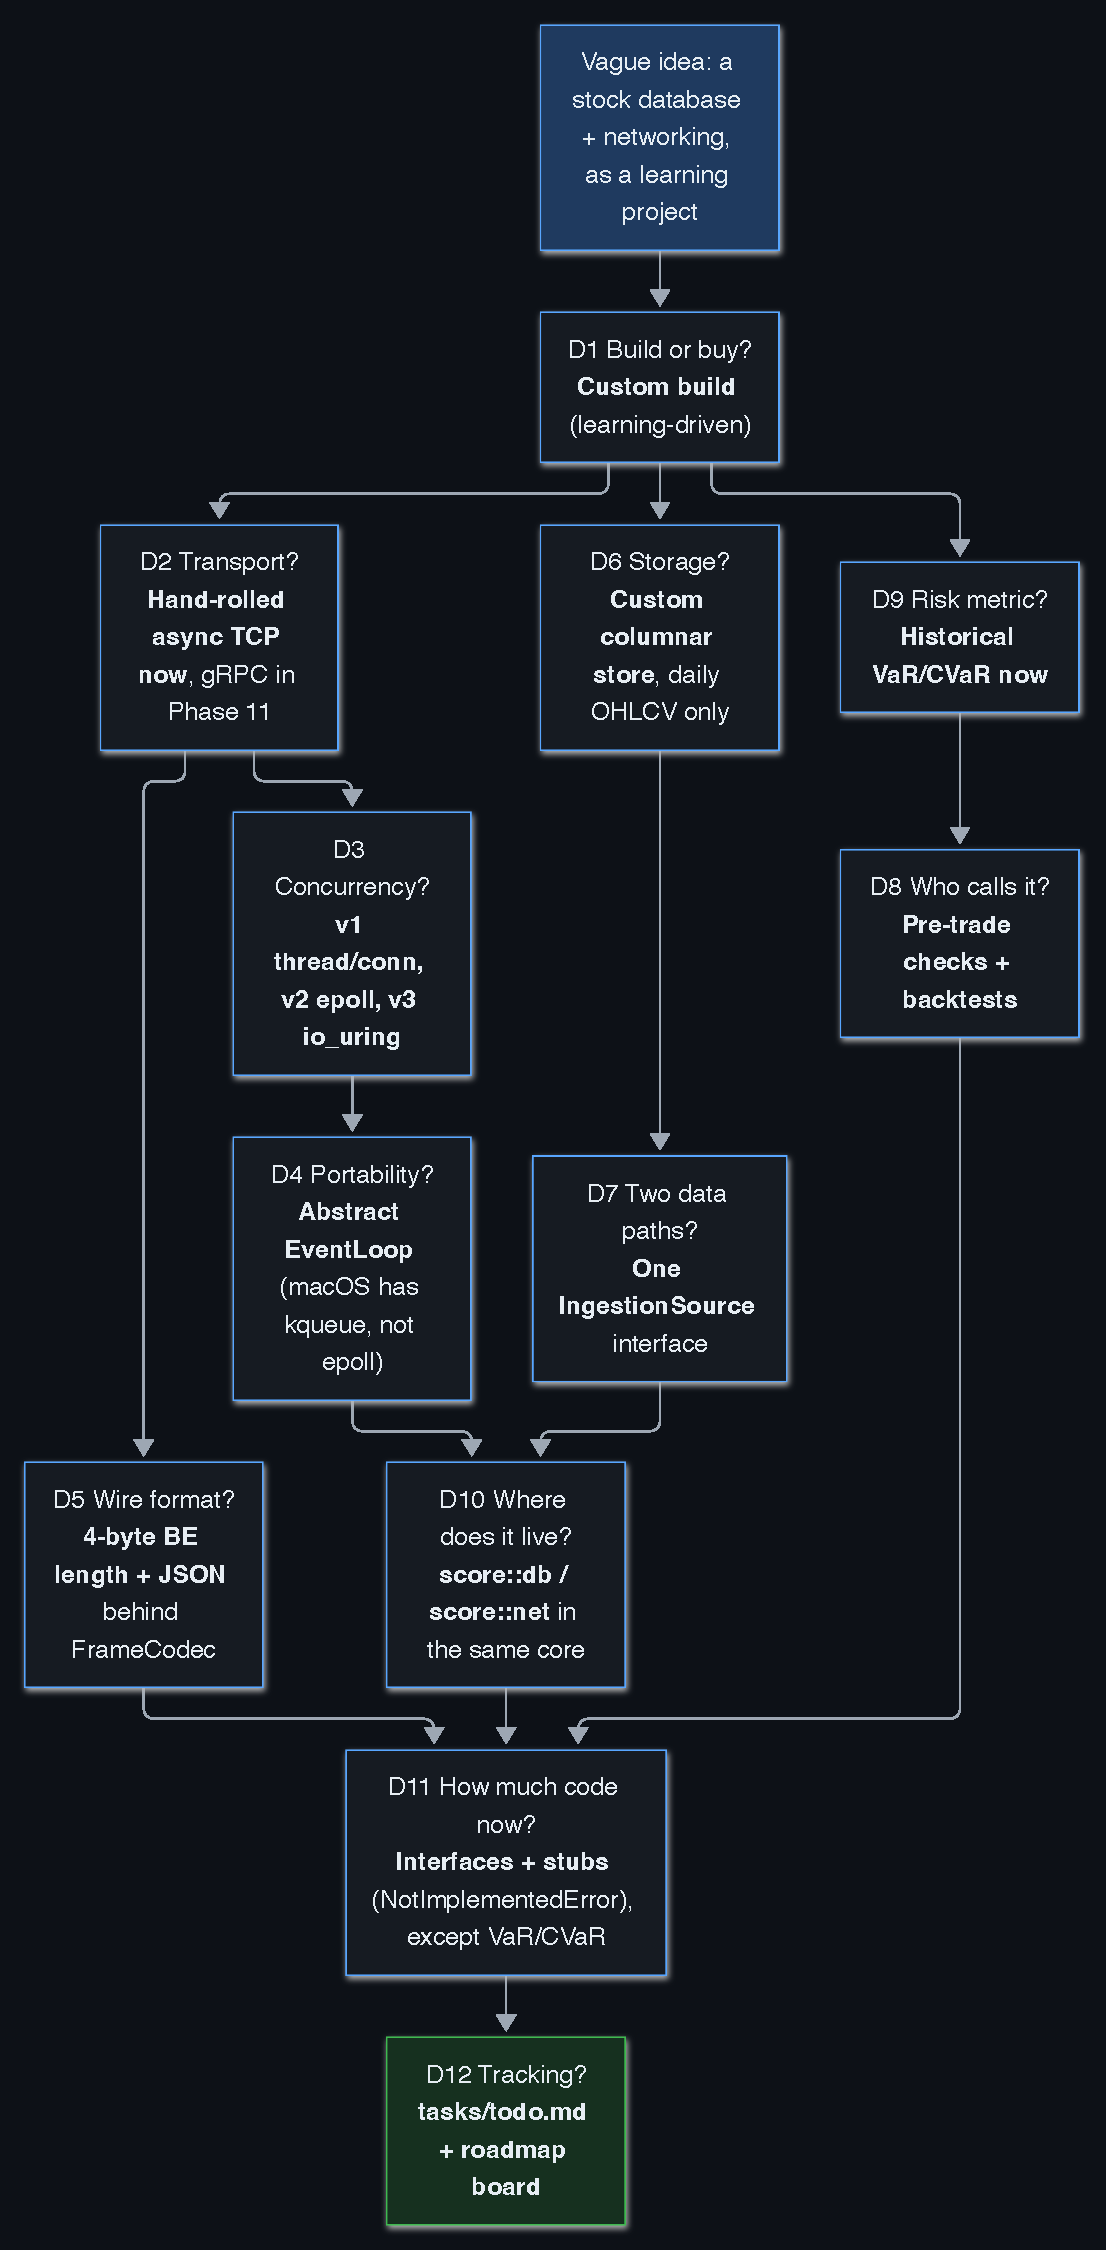
\includegraphics[height=0.82\textheight]{diagrams/grilling.pdf}
\caption{The decision graph of the grilling session (Mermaid). Each node is a question with its recommended answer in
bold. Edges are the dependency relation $\prec$ of \cref{def:frontier}; the session visited nodes in a topological order.}
\label{fig:grill}
\end{figure}

\section{The twelve decisions}
\Cref{tab:decisions} lists the decisions with the alternative that lost and a falsifier for each. Read the
falsifier column carefully: it is the part you will reuse when a decision needs revisiting.

\begin{center}
\footnotesize
\begin{longtable}{@{}>{\leavevmode\bfseries\color{yel}}p{0.6cm} >{\raggedright\arraybackslash}p{3.6cm} >{\raggedright\arraybackslash}p{2.9cm} >{\raggedright\arraybackslash}p{5.4cm}@{}}
\caption{The twelve decisions. ``Lost to'' is the strongest rejected alternative.}\label{tab:decisions}\\
\toprule
\textcolor{muted}{\#} & \textcolor{muted}{Decision} & \textcolor{muted}{Lost to} & \textcolor{muted}{Falsifier (what would reverse it)}\\
\midrule\endfirsthead
\toprule
\textcolor{muted}{\#} & \textcolor{muted}{Decision} & \textcolor{muted}{Lost to} & \textcolor{muted}{Falsifier}\\
\midrule\endhead
D1 & Learning-driven custom build & Off-the-shelf DB + RPC & The goal changes from learning to shipping to users.\\
D2 & Hand-rolled async TCP engine now; gRPC later (Phase 11) & gRPC now & Clients in other languages need the API before Phase 8 is stable.\\
D3 & v1 thread-per-connection $\to$ v2 epoll $\to$ v3 io\_uring (stretch) & Start at epoll & v1 cannot be made correct without the same buffering a reactor needs (\cref{ex:blocking}).\\
D4 & Platform-agnostic \cc{EventLoop} so macOS (kqueue) builds & Linux-only & Development moves entirely to Linux containers.\\
D5 & v1 wire format: 4-byte big-endian length + JSON behind \cc{FrameCodec}; binary later & Binary first & Profiling shows JSON encode/parse dominating request latency.\\
D6 & Custom columnar store, daily OHLCV only & SQLite / Parquet & Intraday or multi-asset data becomes a requirement.\\
D7 & One \cc{IngestionSource} for both data paths & Two ad-hoc loaders & The two sources need incompatible write semantics (e.g.\ corrections that rewrite history).\\
D8 & Users: pre-trade risk checks and backtesting & General analytics & A consumer appears whose queries are not ``one symbol, one date range''.\\
D9 & Real historical VaR/CVaR now & Parametric (Gaussian) VaR & Data too short for the tail ($k=0$, \cref{ch:risk}) at the confidences users ask for.\\
D10 & New \cc{score::db} / \cc{score::net} modules in the same core library & Separate libraries/services & Build times or dependency weight of \texttt{net} hurt Python users who never serve.\\
D11 & Scaffolding only (stubs throw \cc{NotImplementedError}), except VaR/CVaR & Implement everything at once & A stub's interface proves wrong before its implementation phase starts.\\
D12 & Tracked in \file{tasks/todo.md} and the generated roadmap board & Issue tracker & More than one contributor needs to coordinate.\\
\bottomrule
\end{longtable}
\end{center}

\section{Why interfaces first: a counting argument}
Decisions D3, D4 and D5 each name a family of interchangeable implementations: three event loops, two
codecs, two operating systems. Suppose the server were written directly against one concrete loop and one concrete codec.

\begin{proposition}[Sum, not product]\label[proposition]{prop:sum}
Let a component depend on $m$ independent variation points with $v_1,\dots,v_m$ variants each. If it is written against
concrete types, covering all combinations requires $\prod_i v_i$ component variants. If it depends only on an interface per
variation point, it requires one component plus $\sum_i v_i$ implementations.
\end{proposition}
\begin{proof}
Against concrete types, each combination $(a_1,\dots,a_m)$ fixes the source text of the component, and distinct
combinations give distinct texts, hence $\prod_i v_i$ variants. Against interfaces, the component's text mentions no
variant; each variant is written once, behind its interface, and any combination is assembled at construction time
(for \cc{Server}: an \cc{EventLoop&} and a \cc{CodecFactory}). That is $1+\sum_i v_i$ units of code.
\end{proof}

For \texttt{score}, with $v=(3,2)$ for (event loop, codec), that is $6$ server variants versus $1+5$ units, and the gap
widens with every new backend. Parnas made the underlying argument in 1972: decompose a system so that each module
hides one \emph{design decision likely to change}~\cite{parnas1972criteria}. \cc{EventLoop} hides the concurrency model,
\cc{FrameCodec} the wire format, \cc{ColumnStore} the byte layout, \cc{IngestionSource} the provenance of the data.
Martin later named the same idea the Dependency Inversion Principle~\cite{martin2003agile}.

\begin{remarkbox}
Interfaces are not free. Every call through \cc{EventLoop} is a virtual call, and every \cc{IoCallback} is a
\cc{std::function} that may allocate. For a learning project those costs are noise next to a system call, which is
two to three orders of magnitude more expensive (\cref{tab:costs}). Measure before removing them.
\end{remarkbox}

\section{Scaffolding that fails loudly}
Decision D11 says that everything except VaR/CVaR is scaffolding: real headers, real class shapes, and bodies that throw.

\repo[firstline=31,lastline=34]{include/score/core/exceptions.hpp}{The exception every stub throws (lines 31--34). It derives from
\cc{ScoreException}, which derives from \cc{std::runtime_error}, so Python callers see an ordinary exception
once bindings exist.}{lst:notimpl}

\repo{src/net/json_codec.cpp}{A typical stub. Every method throws; none returns a plausible default.}{lst:jsonstub}

\begin{claim}\label[claim]{claim:loud}
A stub that throws is strictly safer than a stub that returns a default value of the declared type.
\end{claim}
\begin{proof}[Argument]
Consider \cc{try_decode()} returning \cc{std::nullopt} as a ``harmless'' default. Every caller treats
\cc{nullopt} as ``not enough bytes yet'', so a test that feeds a complete frame and asserts nothing more than ``no crash''
passes, and a server built on it silently never answers. A throwing stub turns the same test into a failure, and its
message names the unimplemented function. A test can only pass against a throwing stub if it never calls the stub, and that
is visible in coverage. So the throwing stub cannot produce a vacuous pass, while the defaulting stub can.
\end{proof}

\begin{history}
Brooks's advice to ``plan to throw one away''~\cite{brooks1975mythical} is often quoted as permission to write disposable
code. Scaffolding is the opposite bet: keep the \emph{interfaces}, which are cheap to get right by thinking,
and postpone the \emph{implementations}, which are cheap to get right only by building. The grilling session existed to make the
interfaces right before any implementation existed.
\end{history}

\begin{exercises}
\ex{ex:falsify}{\lvA} For decisions D2, D6 and D9, describe a concrete measurement or event in \emph{this} repository that
would trigger the falsifier in \cref{tab:decisions}. Who would observe it, and in which file?

\ex{ex:leak}{\lvB} Parnas's criterion says an interface should hide one secret. \cc{event_loop.hpp} declares
\cc{using SocketHandle = int;}. Which secret leaks through that line? What breaks on Windows, where a socket is
\cc{SOCKET}, an unsigned pointer-sized integer? Propose a fix that does not add a virtual call.

\ex{ex:order}{\lvB} \cc{ColumnStore::append} documents that implementations ``should reject bars that are out of
order or overlap dates already stored''. The interface cannot enforce this. Sketch a type (for example a
\cc{SortedBars} that can only be built by a validating factory) that makes an unsorted batch unrepresentable, and
discuss what it costs at the Python boundary.

\ex{ex:lifetime}{\lvB} \cc{Connection} stores \cc{EventLoop& loop_}, and its destructor is defaulted, while
\cc{close()} must unregister from the loop. Specify the destruction order of \cc{Server}, its \cc{connections_}, and the
loop so that no callback can run on a destroyed \cc{Connection}. Which of the three may outlive the others?

\ex{ex:frontier}{\lvC} \Cref{fig:grill} is one topological order. Find a pair of decisions whose order in the session
could be swapped without changing any answer, and a pair that could not. Then argue whether a design interview
should prefer depth-first (finish a branch) or breadth-first (settle every top-level question first) traversal of the frontier.
\end{exercises}

